%%%%%%%%%%%%%%%%%%%%%%%%%%%%%%%%%%%%%%%%%%%%%%%%%%%%%%%%%%%%%%%
\chapter{3D simulations}\label{}
%%%%%%%%%%%%%%%%%%%%%%%%%%%%%%%%%%%%%%%%%%%%%%%%%%%%%%%%%%%%%%%



%%%%%%%%%%%%%%%%%%%%%%%%%%%%%%%%%%%%%%%%%%%%%%%%%%%%%%%%%%%%%%%
\section{Maps: Geomorphologic maps}
%%%%%%%%%%%%%%%%%%%%%%%%%%%%%%%%%%%%%%%%%%%%%%%%%%%%%%%%%%%%%%%
\begin{figure}[!htbp]
\begin{center}
  \begin{minipage}[c]{1.0\textwidth}
  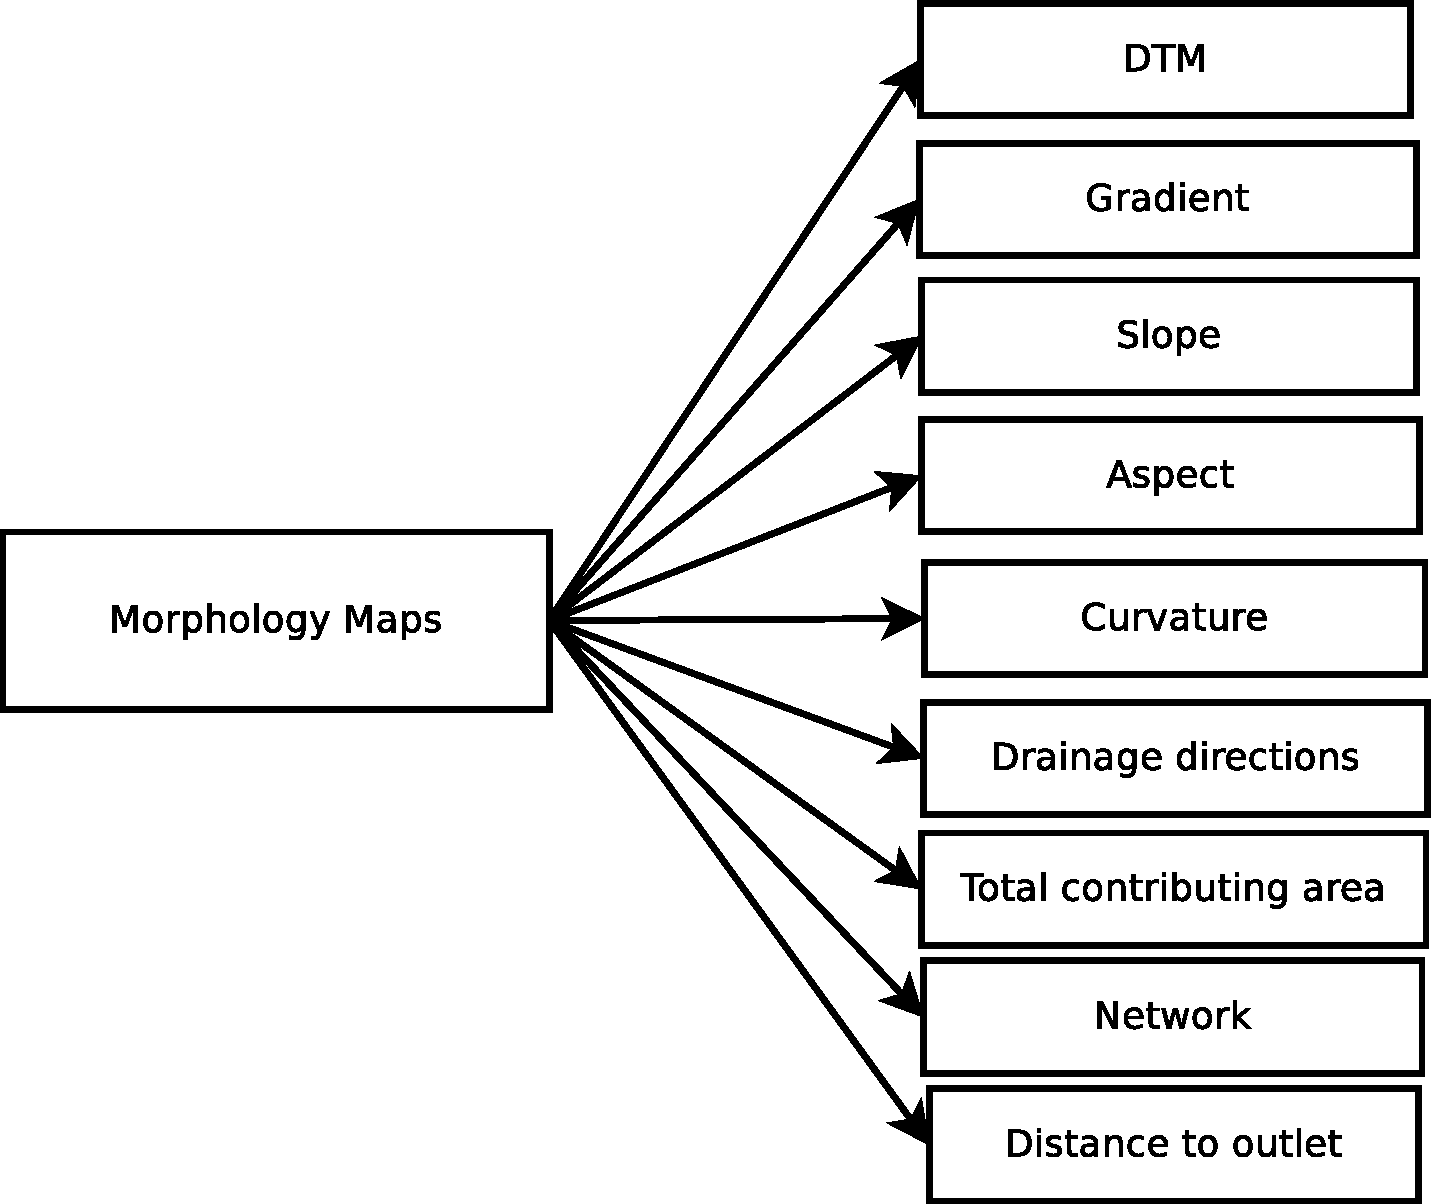
\includegraphics[width=0.9\textwidth]{./images/pic_3D/morpho_vert_1.pdf}
  \end{minipage}
\end{center}
\textsl{\caption{morphology}\label{}}
\end{figure}

\begin{table}[!h]
\begin{center}
\begin{tabular}{llll}
\hline
\textbf{MAP}            &   \textbf{UNIT OF} &    \textbf{RANGE OF}         &     \textbf{JGRASS}           \\
\textbf{}               &   \textbf{MEASURE} &    \textbf{VALUE}            &     \textbf{ORIGIN}           \\
\hline 
\hline
DTM                     &    [m a.s.l]               &       [0-8848]		    &           			   \\             
Gradient	        &     [degree]               &        [0-90]   		    &     \textsl{h.gradient}       			   \\
Slope                   &     [degree]               &       [0-90]		    &     \textsl{h.slope}           \\ 
Aspect                  &     [degree]               &		0 at north	    &     \textsl{h.aspect}   \\ 
			&     		             &     measured clockwise       &     \textsl{h.aspect}   \\ 
Curvature               &        [-]                 &        0 concave  	    &     \textsl{h.curvature}                \\ 
			&                            &        1 convex  	    &     \textsl{h.curvature}                \\ 
Drainage direction      &         [-]         	     &  [1..8]      		    &     \textsl{h.draindir}                   		     \\
Total contributing area &     [$m^2$]                &          [0-..] 		    &     \textsl{h.tca}    \\ 
Network map             &            [-]             &         0 slope		    &     \textsl{h.extractnetwork}                 \\
			&                            &        10 channel  	    &     \textsl{h.curvature}                \\ 
Distance to outlet      &       [m]                  &          [0-..]		    &     \textsl{h.d2o3d}            				\\
Sky view factor         &       [-]                  &          [0..1]		    &     calculated by GEOtop                 \\ 
\hline
\end{tabular}
\textsl{\caption{Input morphology map in \textit{GEOtop}}}
 \label{}
 \end{center}
\end{table}


\newpage
%=============================================================%
\subsection{DTM}
%=============================================================%
The Digital Terrain Model is a digital representation of ground surface topography or terrain. 
The input format required for GEOtop is the ESRII ASCII format, which header is
expressed as:
\begin{table}[!h]
\begin{footnotesize}
\begin{center}
\begin{tabular}{lc}
  \hline
ncols   &      ..\\
nrows    &     ..\\
xllcorner  &   ..\\
yllcorner   &  ..\\
cellsize   &   ..\\
NODATA\_value & ..\\
  \hline
\end{tabular}
\textsl{\caption{ESRII ASCII header}}\label{}
\end{center}
\end{footnotesize}
\end{table}

\begin{figure}[h!]
\begin{center}
  \begin{minipage}[c]{.25\textwidth}
    \centering
    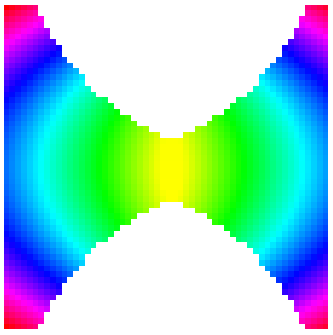
\includegraphics[width=1\textwidth]{./images/user/dem.png}
  \end{minipage}%
  \hspace{10mm}%
  \begin{minipage}[c]{.40\textwidth}
    \centering
    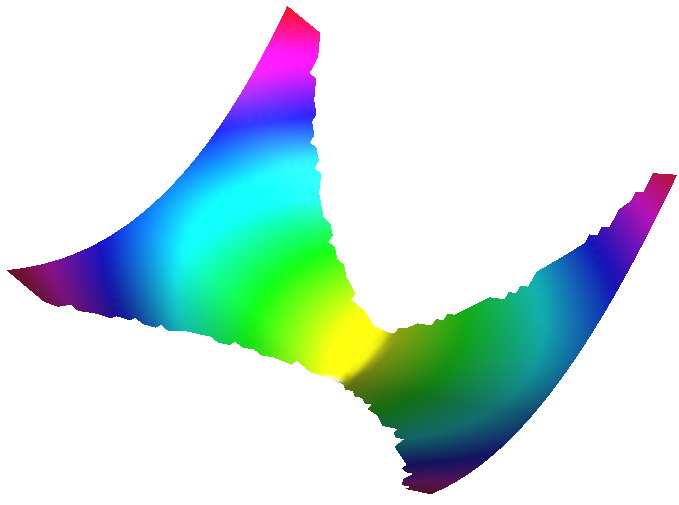
\includegraphics[width=1\textwidth]{./images/user/dem_3D.png}
  \end{minipage}
  \begin{minipage}[c]{.10\textwidth}
    \centering
    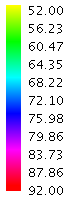
\includegraphics[width=1\textwidth]{./images/user/dem_legenda.png}
  \end{minipage}
\end{center}
\textsl{\caption{DTM}\label{}}
\end{figure}



%\begin{figure}[!htbp]
% \centering
% \subfigure[DTM]
%   {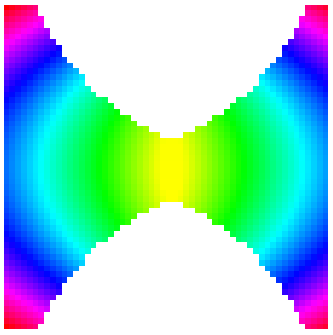
\includegraphics[width=0.25\textwidth]{./images/user/dem.png}}
%\hspace{5mm}
% \subfigure[DTM 3D]
%   {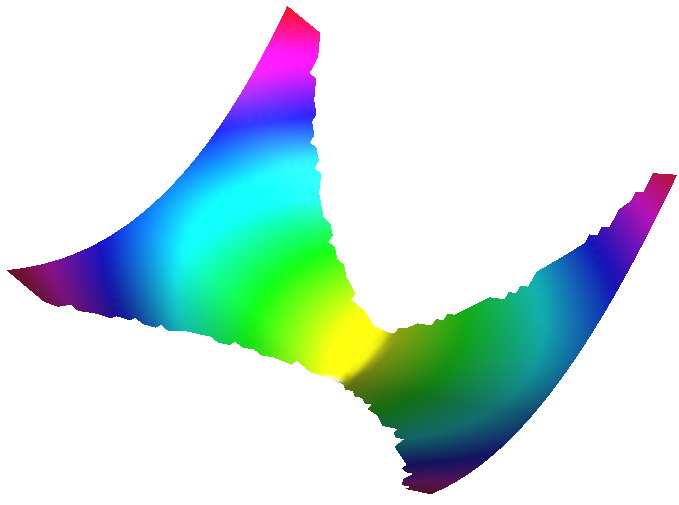
\includegraphics[width=0.4\textwidth]{./images/user/dem_3D.png}}
%\hspace{5mm}
% \subfigure[elevation (m)]
%   {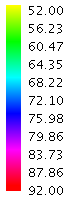
\includegraphics[width=0.1\textwidth]{./images/user/dem_legenda.png}}
%\end{figure}
%=============================================================%
\subsection{Gradient}
%=============================================================%
The gradient map is the map with the slope angle in each point of the map.
The gradient is:
\begin{equation}
\nabla z = (f_x,f_y)
\end{equation}
Where 
\begin{equation}
f_x =\frac{\partial z}{\partial x}  \hspace{4em}f_y=\frac{\partial z}{\partial y}
\end{equation}



Indicating with:
\begin{equation}
f_x =\frac{\partial z}{\partial x}  \hspace{4em}f_y
=\frac{\partial z}{\partial y}
\end{equation}

and:
\begin{equation}
p = f_x^2 + f^2_y
\end{equation}

\begin{itemize}
\item The gradient is:
\begin{equation}
\nabla z = (f_x,f_y)
\end{equation}
\item the maximum-slope (the slope) angle is:
\begin{equation}
\gamma =\arctan \sqrt{p}
\end{equation}
\item and the aspect (measured counterclockwise from the "x" axis) is:
\begin{equation}
\alpha = \arctan \frac{f_y}{f_x}
\end{equation}
\end{itemize}
\noindent From the gradient map, we deduce the drainage directions which correspond (up to
inertial effects negligible at first approximation) to the water flows. \\






\begin{figure}[h!]
\begin{center}
  \begin{minipage}[c]{.25\textwidth}
    \centering
    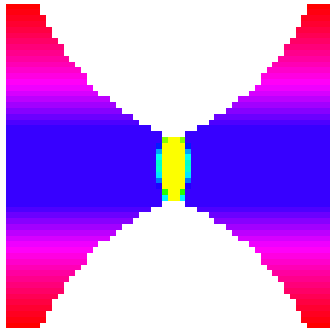
\includegraphics[width=1\textwidth]{./images/user/slope.png}
  \end{minipage}%
  \hspace{10mm}%
  \begin{minipage}[c]{.40\textwidth}
    \centering
    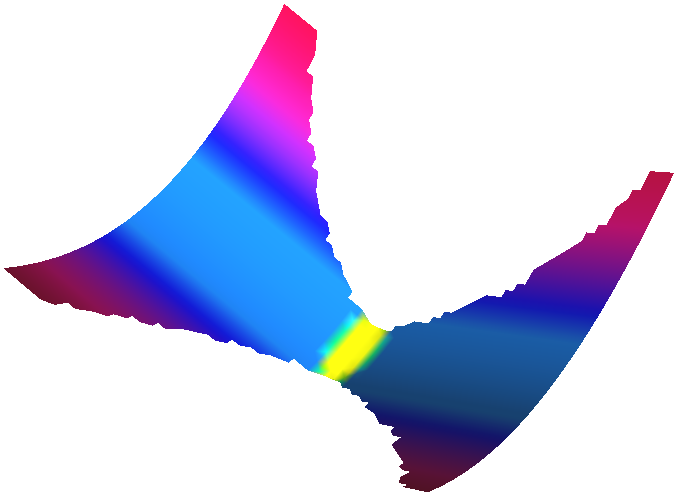
\includegraphics[width=1\textwidth]{./images/user/slope_3D.png}
  \end{minipage}
  \begin{minipage}[c]{.10\textwidth}
    \centering
    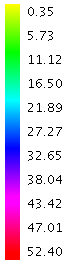
\includegraphics[width=1\textwidth]{./images/user/slope_legenda.png}
  \end{minipage}
\end{center}
\textsl{\caption{Gradient}\label{}}
\end{figure}


%=============================================================%
\subsection{Slope}
%=============================================================%
The slope map estimates the slope in every site
by employing the drainage directions. Differently from the
gradients, slope calculates the drop between each pixel and the
adjacent points placed underneath and it divides the result by the
pixel length or by the length of the pixel diagonal, according to
the cases. The greatest value is the one chosen as slope.
The slope map is relevant from many points of view. 
Since the main motive-power of the hydrologic flows on the Earth's surface and in the soil
directly below is gravity, the surface gradient identifies, in first
approximation, the water flow directions and contributes to the determination of
their speed.
The sub-surface flow is proportional to slope; the surface runoff
to the root of the slope. 
Also the erosion and the consequent solid transport
depend on the gradients of the topographic surfaces: these have components which
are proportional to the gradients both in a linear and in a non-linear way; 
% [e.g.\cite{Scheidegger1991}]
moreover, zones with a great slope are generally devoid
of soil and they represent zones of exposed rock.  \\

\begin{figure}[h!]
\begin{center}
  \begin{minipage}[c]{.25\textwidth}
    \centering
    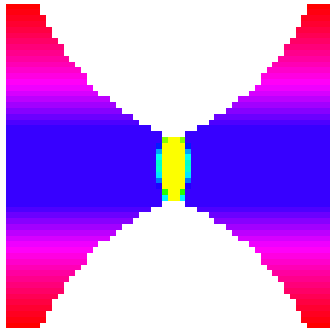
\includegraphics[width=1\textwidth]{./images/user/slope.png}
  \end{minipage}%
  \hspace{10mm}%
  \begin{minipage}[c]{.40\textwidth}
    \centering
    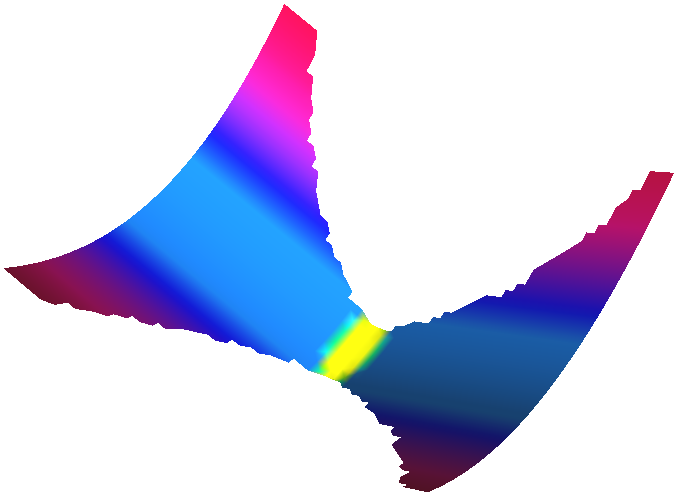
\includegraphics[width=1\textwidth]{./images/user/slope_3D.png}
  \end{minipage}
  \begin{minipage}[c]{.10\textwidth}
    \centering
    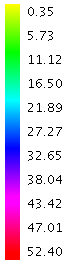
\includegraphics[width=1\textwidth]{./images/user/slope_legenda.png}
  \end{minipage}
\end{center}
\textsl{\caption{Slope}\label{}}
\end{figure}

%\begin{figure}[!htbp]
% \centering
% \subfigure[slope]
%   {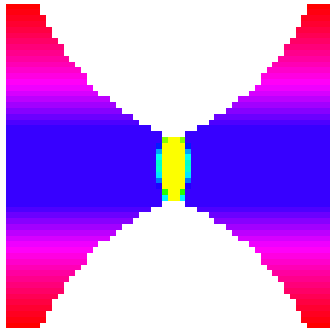
\includegraphics[width=0.25\textwidth]{./images/user/slope.png}}
%\hspace{5mm}
% \subfigure[slope 3D]
%   {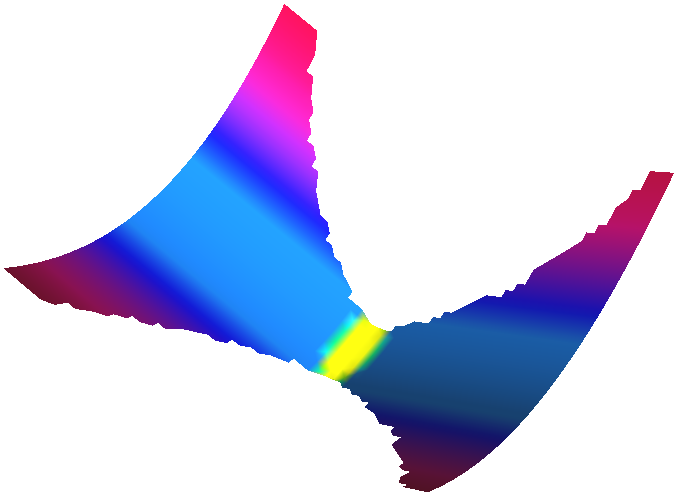
\includegraphics[width=0.4\textwidth]{./images/user/slope_3D.png}}
%\hspace{5mm}
% \subfigure[\textdegree]
%   {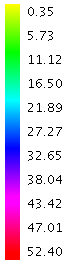
\includegraphics[width=0.1\textwidth]{./images/user/slope_legenda.png}}
%\end{figure}




%=============================================================%
\subsection{Aspect}
%=============================================================%
The aspect map extimates the
inclination angle of the gradient by considering a reference system
which puts the zero towards the east and the rotation angle
anticlockwise. The unit of measure is degree. It differs from the drainage directions in which it
is given in radiants and it is a continuous function while drainage
direction returns a number between 1 and 10. The aspect is 0 in the the
South direction and increase clockwise.\\

\begin{figure}[!h]
\begin{center}
  \begin{minipage}[c]{.25\textwidth}
    \centering
    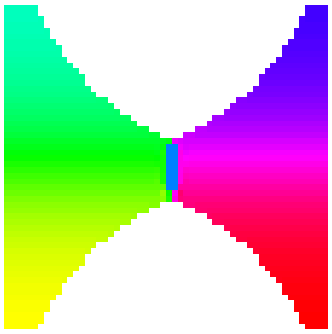
\includegraphics[width=1\textwidth]{./images/user/aspect.png}
  \end{minipage}%
  \hspace{10mm}%
  \begin{minipage}[c]{.40\textwidth}
    \centering
    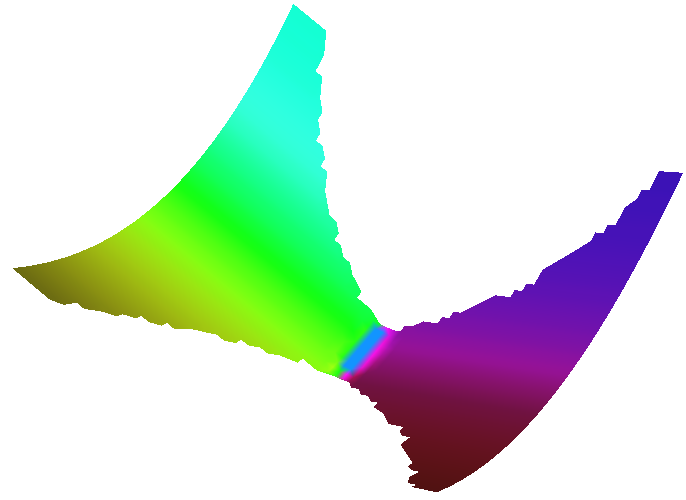
\includegraphics[width=1\textwidth]{./images/user/aspect_3D.png}
  \end{minipage}
  \begin{minipage}[c]{.10\textwidth}
    \centering
    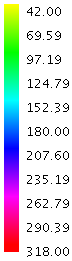
\includegraphics[width=1\textwidth]{./images/user/aspect_legenda.png}
  \end{minipage}
\end{center}
\textsl{\caption{Aspect}\label{}}
\end{figure}


%\begin{figure}[!htbp]
% \centering
% \subfigure[aspect]
%   {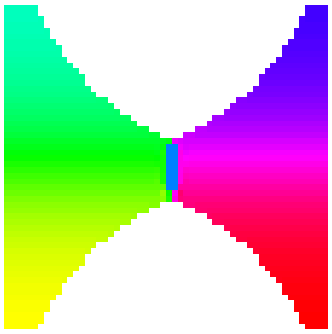
\includegraphics[width=0.25\textwidth]{./images/user/aspect.png}}
%\hspace{5mm}
% \subfigure[aspect 3D]
%   {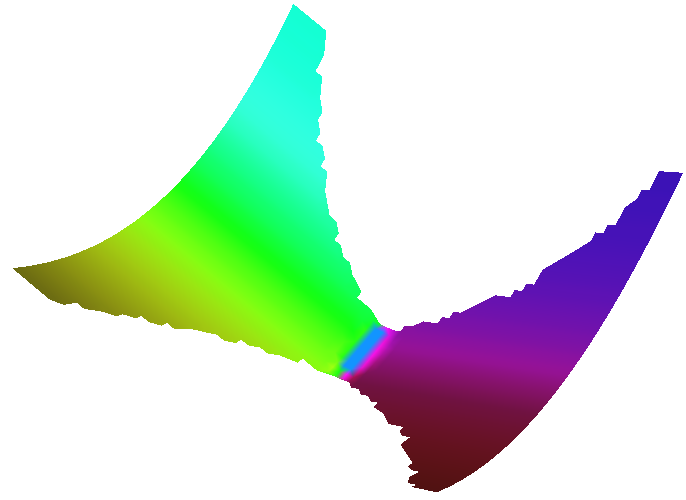
\includegraphics[width=0.4\textwidth]{./images/user/aspect_3D.png}}
%\hspace{5mm}
% \subfigure[\textdegree]
%   {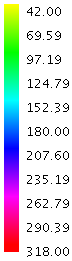
\includegraphics[width=0.1\textwidth]{./images/user/aspect_legenda.png}}
%\end{figure}


%=============================================================%
\subsection{Curvature}
%=============================================================%
The curvatures represent the deviations of the gradient vector for unit length
(in radiants) along particular curves plotted on the surface under
consideration. In particular, the presence of non-zero curvatures has relevant
effects on the representation of the properties of the surfaces discretized. For
example, if the surface has a negative normal curvature, then the gradients have
diverging directions at the extremes of the pixel, $P$, and the contributing
area in $P$ is spread over several adjacent pixels: in this case topography is
called locally divergent. Vice versa, the surface is locally converging
(negative curvature) and the contributing area in $P$ tends to be spread over a
limited set of adjacent pixels and almost centainly on a single pixel. 
Roughly speaking, the convex zones are hillslope zones, the concave zones are
valleys. As it is known, the latter contain the channel network. Then, the
curvature tends to discriminate the points across the basin with greater
humidity content (the concave ones). This fact has relevant consequences on the
overall hydrologic behavior of basins and, in particular, on the production of
runoff and on the evapotranspiration distribution. \\
The Laplace operator, which here represents the curvature, is defined by:
\begin{equation}
\nabla^2 z = \frac{\partial^2 \ z}{\partial x^2} + \frac{\partial^2
\ z}{\partial y^2}
\end{equation}\label{nabla}
and it makes it possible to distinguish the convex zones ($\nabla^2 z  < 0$)
from concave zones ($\nabla^2 z >0$) or planar zones ($\nabla^2 z \sim 0$).  

\begin{figure}[h!]
\begin{center}
  \begin{minipage}[c]{.25\textwidth}
    \centering
    
\includegraphics[width=1\textwidth]{./images/user/curvature.png}
  \end{minipage}%
  \hspace{10mm}%
  \begin{minipage}[c]{.40\textwidth}
    \centering
    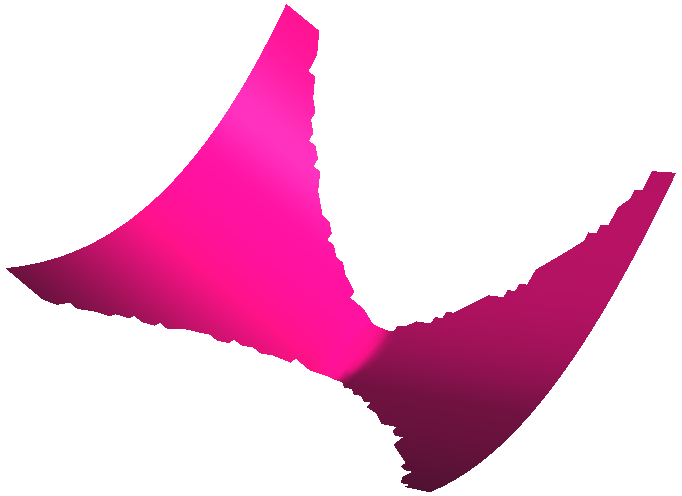
\includegraphics[width=1\textwidth]{./images/user/curvature_3D.png}
  \end{minipage}
  \begin{minipage}[c]{.10\textwidth}
    \centering
    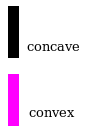
\includegraphics[width=1\textwidth]{./images/user/curvature_legenda.png}
  \end{minipage}
\end{center}
\textsl{\caption{Curvature}\label{}}
\end{figure}

%\begin{figure}[!htbp]
% \centering
% \subfigure[profile curvature]
%   {
\includegraphics[width=0.25\textwidth]{./images/user/curvature.png}}
%\hspace{5mm}
% \subfigure[profile curvature 3D]
%   {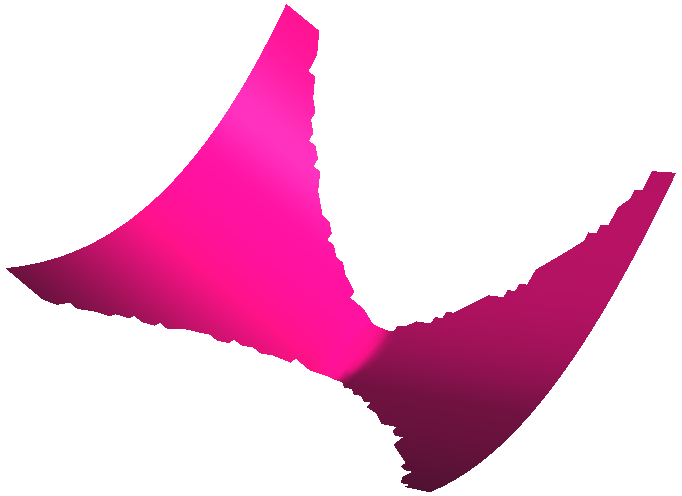
\includegraphics[width=0.4\textwidth]{./images/user/curvature_3D.png}}
%\hspace{5mm}
% \subfigure[legend]
%   {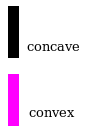
\includegraphics[width=0.1\textwidth]{./images/user/curvature_legenda.png}}
%\end{figure}




%=============================================================%
\subsection{Drainage directions}
%=============================================================%
The drainage directions map calculates the drainage directions
minimizing the deviation from the real flow. The deviation is
calculated using a triangular construction and it must be given in
degrees. The deviation could be cumulated along the path using the $\lambda$
parameter, and when it assumes a limit value the flux is redirect
toward the real gradient direction. 
If the drainage network is known and marked in a raster matrix, its flow 
directions can be kept fixed.\\

\begin{figure}[h!]
\begin{center}
  \begin{minipage}[c]{.25\textwidth}
    \centering
    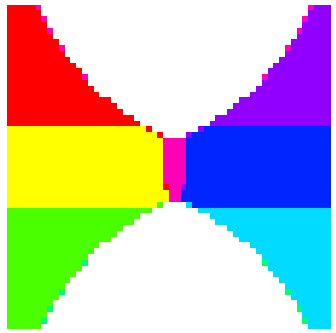
\includegraphics[width=1\textwidth]{./images/user/drenaggio.png}
  \end{minipage}%
  \hspace{10mm}%
  \begin{minipage}[c]{.40\textwidth}
    \centering
    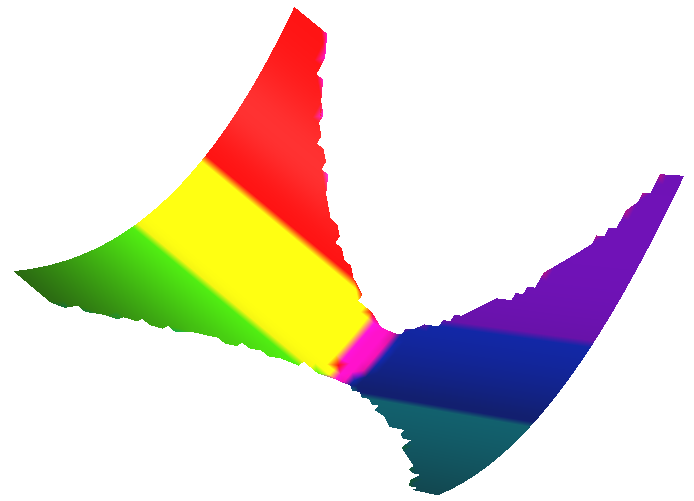
\includegraphics[width=1\textwidth]{./images/user/drenaggio_3D.png}
  \end{minipage}
  \begin{minipage}[c]{.10\textwidth}
    \centering
    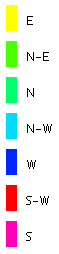
\includegraphics[width=1\textwidth]{./images/user/drenaggio_legenda.png}
  \end{minipage}
\end{center}
\textsl{\caption{Drainage directions}\label{}}
\end{figure}

%\begin{figure}[!htbp]
% \centering
% \subfigure[drainage directions]
%   {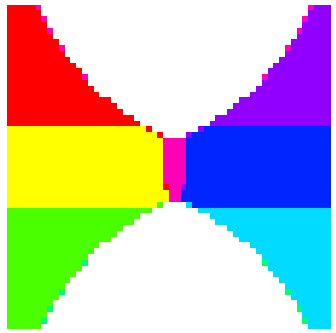
\includegraphics[width=0.25\textwidth]{./images/user/drenaggio.png}}
%\hspace{5mm}
% \subfigure[draiange directions 3D]
%   {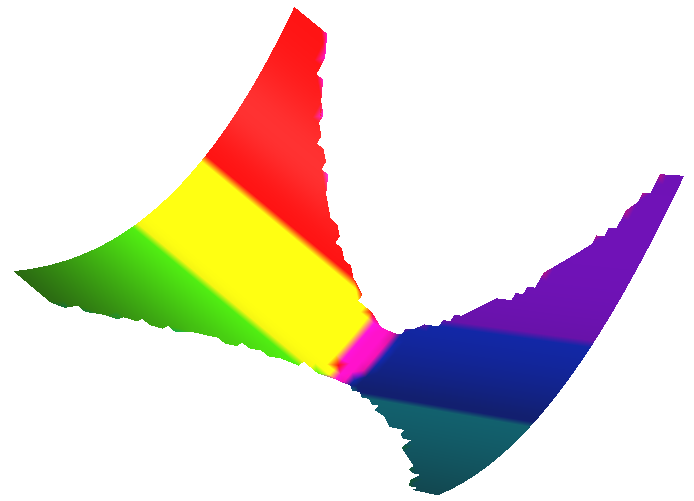
\includegraphics[width=0.4\textwidth]{./images/user/drenaggio_3D.png}}
%\hspace{5mm}
% \subfigure[legend]
%{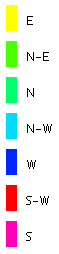
\includegraphics[width=0.08\textwidth]{./images/user/drenaggio_legenda.png}}
%\end{figure}


%=============================================================%
\subsection{Total contributing area}
%=============================================================%
The Total Contributing Area represent the planar
projection  of the areas afferent to a point in the basin. Once the drainage
directions have been defined, is possible to calculate, for each site, the
total drainage area afferent to it.
The number of sites draining in the $i$-esimal element determines the total 
area $A_i$ which can be expressed as follows:
\begin{equation}
A_i =\sum_{j\:\in\: nn(i)} W_{ij}A_{j} + R_{i}
\end{equation}
where $nn(i)$ represents the set of the eight (six, four or three) pixels
surrounding  the $i$-esimal site; $R_i$ is the area of every pixel.
The total cumulative area is an extremely important quantity in the
geomorphologic  and hydrologic study of a river basin: indeed, it seems to be
strictly related to the discharge flowing into the different points of the
system in uniform precipitation conditions.\\

\begin{figure}[h!]
\begin{center}
  \begin{minipage}[c]{.25\textwidth}
    \centering
    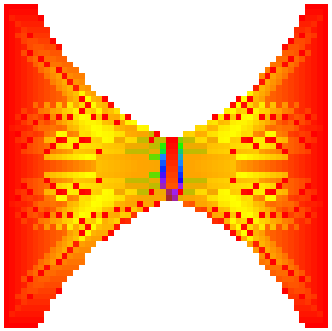
\includegraphics[width=1\textwidth]{./images/user/area.png}
  \end{minipage}%
  \hspace{10mm}%
  \begin{minipage}[c]{.40\textwidth}
    \centering
    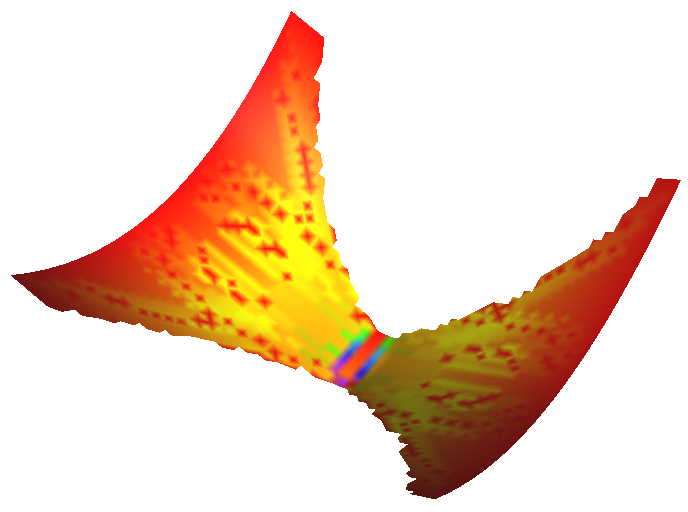
\includegraphics[width=1\textwidth]{./images/user/area_3D.png}
  \end{minipage}
  \begin{minipage}[c]{.10\textwidth}
    \centering
    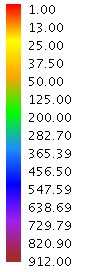
\includegraphics[width=1\textwidth]{./images/user/area_legenda.png}
  \end{minipage}
\end{center}
\textsl{\caption{Total contributing area}\label{}}
\end{figure}

%\begin{figure}[!htbp]
% \centering
%% \subfigure[contributing area]
%   {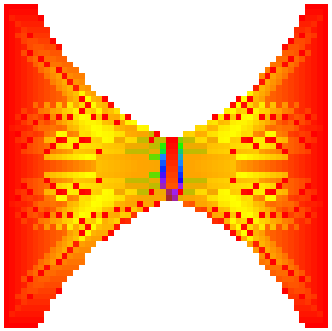
\includegraphics[width=0.25\textwidth]{./images/user/area.png}}
%\hspace{5mm}
%% \subfigure[contributing area 3D]
%   {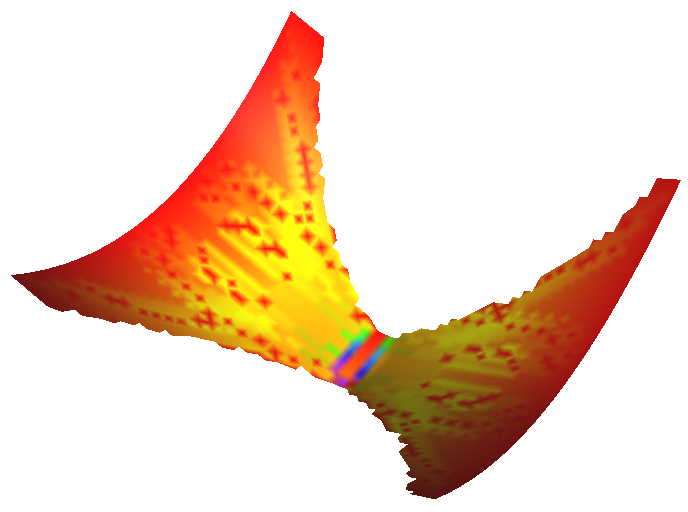
\includegraphics[width=0.4\textwidth]{./images/user/area_3D.png}}
%\hspace{5mm}
%% \subfigure[$(m^2)$ ]
%   {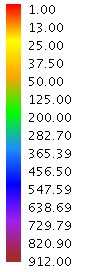
\includegraphics[width=0.1\textwidth]{./images/user/area_legenda.png}}
%\end{figure}


Note that the total contributing area map is used only if the channel network 
is not given as a input map. GEOtop in fact has his own subroutines to automatic calculated
the morphology maps.

%=============================================================%
\subsection{Network}
%=============================================================%
The network map is a map containing all the channel network of the basin.

\begin{figure}[h!]
\begin{center}
  \begin{minipage}[c]{.25\textwidth}
    \centering
    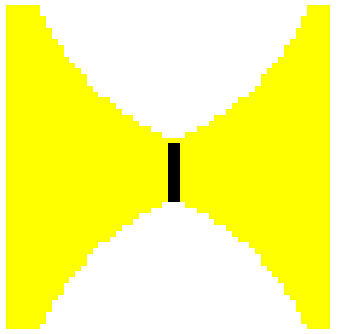
\includegraphics[width=1\textwidth]{./images/user/reticolo.png}
  \end{minipage}%
  \hspace{10mm}%
  \begin{minipage}[c]{.40\textwidth}
    \centering
    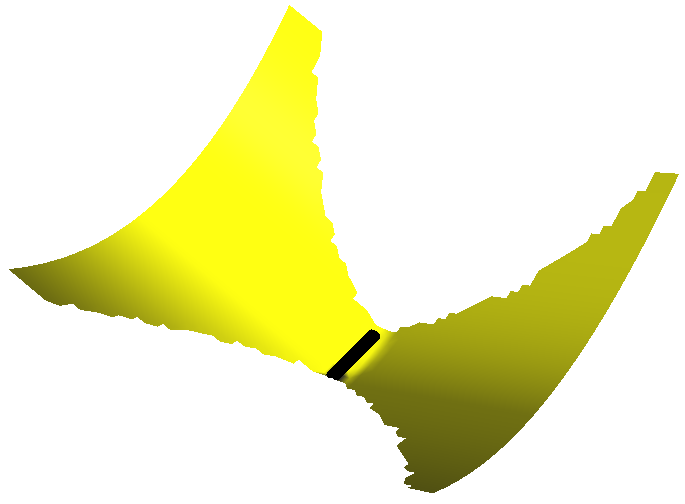
\includegraphics[width=1\textwidth]{./images/user/reticolo_3D.png}
  \end{minipage}
  \begin{minipage}[c]{.10\textwidth}
    \centering
    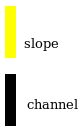
\includegraphics[width=1\textwidth]{./images/user/reticolo_legenda.png}
  \end{minipage}
\end{center}
\textsl{\caption{Network}\label{}}
\end{figure}

%\begin{figure}[!htbp]
% \centering
% \subfigure[stream network]
%   {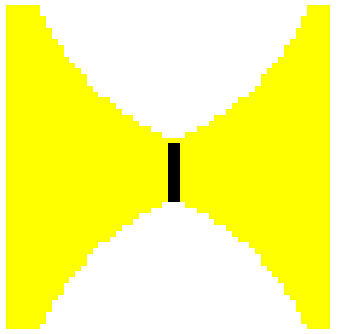
\includegraphics[width=0.25\textwidth]{./images/user/reticolo.png}}
%\hspace{5mm}
% \subfigure[stream network]
%   {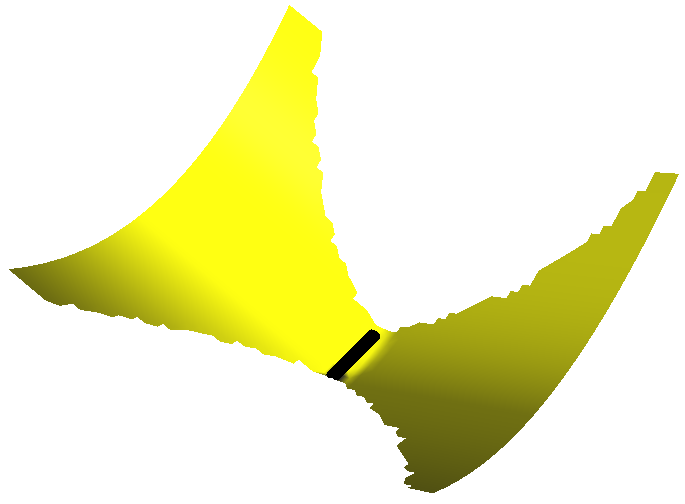
\includegraphics[width=0.4\textwidth]{./images/user/reticolo_3D.png}}
%\hspace{5mm}
% \subfigure[legend]
%   {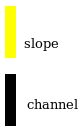
\includegraphics[width=0.1\textwidth]{./images/user/reticolo_legenda.png}}
%\end{figure}

%=============================================================%
\subsection{Distance to outlet}
%=============================================================%
The distance to outlet map is the map of the euclidean distance of each pixel from the outlet
of the bigger basin which contains it.

\begin{figure}[h!]
\begin{center}
  \begin{minipage}[c]{.25\textwidth}
    \centering
    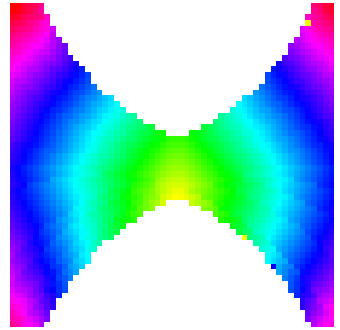
\includegraphics[width=1\textwidth]{./images/user/distance.png}
  \end{minipage}%
  \hspace{10mm}%
  \begin{minipage}[c]{.40\textwidth}
    \centering
    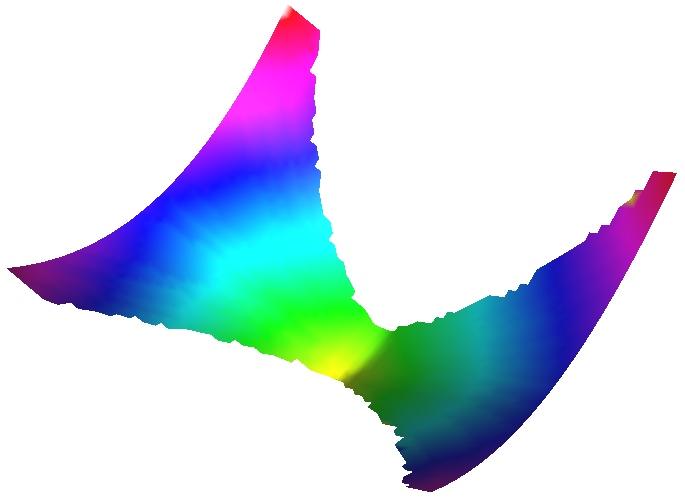
\includegraphics[width=1\textwidth]{./images/user/distance_3D.png}
  \end{minipage}
  \begin{minipage}[c]{.10\textwidth}
    \centering
    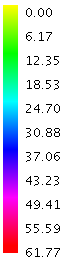
\includegraphics[width=1\textwidth]{./images/user/distance_legenda.png}
  \end{minipage}
\end{center}
\textsl{\caption{Distance to outlet}\label{}}
\end{figure}


% \begin{figure}[!htbp]
% \centering
% \subfigure[outlet]
%   {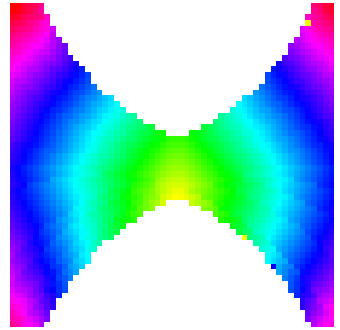
\includegraphics[width=0.25\textwidth]{./images/user/distance.png}}
%\hspace{5mm}
% \subfigure[outlet 3D]
%   {\includegraphics[width=0.4\textwidth]{./images/user/distance_3D.png}}
%\hspace{5mm}
% \subfigure[(m)]
%   {\includegraphics[width=0.09\textwidth]{./images/user/distance_legenda.png}}
%\end{figure}


%=============================================================%
\subsection{Sky view factor}
%=============================================================%
The sky view
factor is the angular fraction of sky visible from a point.
Without obstructions, the factor is 1 and in a mountain
environment the factor can be less than 0.6 and it can be important
to take it in account for evaluating the diffuse solar radiation. The
sky view factor is calculated separately with the program
\emph{Sky.c}(Verardo, 1998).
The sky view factor is 1 in a flat area and it decreases in a
valley, where the hillslope covers a portion of the sky.\\

%\begin{figure}[h!]
%\begin{center}
%  \begin{minipage}[c]{.25\textwidth}
%    \centering
%    \includegraphics[width=1\textwidth]{./images/user/sky.png}
%  \end{minipage}%
%  \hspace{10mm}%
%  \begin{minipage}[c]{.40\textwidth}
%    \centering
%    \includegraphics[width=1\textwidth]{./images/user/sky_3D.png}
%  \end{minipage}
%  \begin{minipage}[c]{.10\textwidth}
%    \centering
%    \includegraphics[width=1\textwidth]{./images/user/sky_legenda.png}
%  \end{minipage}
%\end{center}
%\textsl{\caption{Distance to outlet}\label{}}
%\end{figure}


\newpage
%%%%%%%%%%%%%%%%%%%%%%%%%%%%%%%%%%%%%%%%%%%%%%%%%%%%%%%%%%%%%%%
\section{Maps: Additional maps}
%%%%%%%%%%%%%%%%%%%%%%%%%%%%%%%%%%%%%%%%%%%%%%%%%%%%%%%%%%%%%%%
\begin{figure}[!htbp]
\begin{center}
  \begin{minipage}[c]{1.0\textwidth}
  \includegraphics[width=0.9\textwidth]{./images/diagrammi/Additional.pdf}
  \end{minipage}
\end{center}
\textsl{\caption{additional}\label{}}
\end{figure}
In this section will be listed and explained the two additional maps
required. They are:
\begin{itemize}
 \item Land cover
 \item Soil stratigraphy
\end{itemize}

%\newpage
%=============================================================%
\subsection{Land cover}
%=============================================================%
The Land cover map is a map with the different land cover type of the basin.
It is linked with the roughness, the vegetation height and the color of the cover.

\begin{figure}[h!]
\begin{center}
  \begin{minipage}[c]{.25\textwidth}
    \centering
    \includegraphics[width=1\textwidth]{./images/user/sky_.png}
  \end{minipage}%
  \hspace{10mm}%
  \begin{minipage}[c]{.40\textwidth}
    \centering
    \includegraphics[width=1\textwidth]{./images/user/sky_3D_.png}
  \end{minipage}
  \begin{minipage}[c]{.10\textwidth}
    \centering
    \includegraphics[width=1\textwidth]{./images/user/sky_legenda_.png}
  \end{minipage}
\end{center}
\textsl{\caption{Land cover map}\label{}}
\end{figure}

%\newpage
